\documentclass[noauthor,nooutcomes,hints,handout]{ximera}

\graphicspath{  
{./}
{./whoAreYou/}
{./drawingWithTheTurtle/}
{./bisectionMethod/}
{./circles/}
{./anglesAndRightTriangles/}
{./lawOfSines/}
{./lawOfCosines/}
{./plotter/}
{./staircases/}
{./pitch/}
{./qualityControl/}
{./symmetry/}
{./nGonBlock/}
}


%% page layout
\usepackage[cm,headings]{fullpage}
\raggedright
\setlength\headheight{13.6pt}


%% fonts
\usepackage{euler}

\usepackage{FiraMono}
\renewcommand\familydefault{\ttdefault} 
\usepackage[defaultmathsizes]{mathastext}
\usepackage[htt]{hyphenat}

\usepackage[T1]{fontenc}
\usepackage[scaled=1]{FiraSans}

%\usepackage{wedn}
\usepackage{pbsi} %% Answer font


\usepackage{cancel} %% strike through in pitch/pitch.tex


%% \usepackage{ulem} %% 
%% \renewcommand{\ULthickness}{2pt}% changes underline thickness

\tikzset{>=stealth}

\usepackage{adjustbox}

\setcounter{titlenumber}{-1}

%% journal style
\makeatletter
\newcommand\journalstyle{%
  \def\activitystyle{activity-chapter}
  \def\maketitle{%
    \addtocounter{titlenumber}{1}%
                {\flushleft\small\sffamily\bfseries\@pretitle\par\vspace{-1.5em}}%
                {\flushleft\LARGE\sffamily\bfseries\thetitlenumber\hspace{1em}\@title \par }%
                {\vskip .6em\noindent\textit\theabstract\setcounter{question}{0}\setcounter{sectiontitlenumber}{0}}%
                    \par\vspace{2em}
                    \phantomsection\addcontentsline{toc}{section}{\thetitlenumber\hspace{1em}\textbf{\@title}}%
                     }}
\makeatother



%% thm like environments
\let\question\relax
\let\endquestion\relax

\newtheoremstyle{QuestionStyle}{\topsep}{\topsep}%%% space between body and thm
		{}                      %%% Thm body font
		{}                              %%% Indent amount (empty = no indent)
		{\bfseries}            %%% Thm head font
		{)}                              %%% Punctuation after thm head
		{ }                           %%% Space after thm head
		{\thmnumber{#2}\thmnote{ \bfseries(#3)}}%%% Thm head spec
\theoremstyle{QuestionStyle}
\newtheorem{question}{}



\let\freeResponse\relax
\let\endfreeResponse\relax

%% \newtheoremstyle{ResponseStyle}{\topsep}{\topsep}%%% space between body and thm
%% 		{\wedn\bfseries}                      %%% Thm body font
%% 		{}                              %%% Indent amount (empty = no indent)
%% 		{\wedn\bfseries}            %%% Thm head font
%% 		{}                              %%% Punctuation after thm head
%% 		{3ex}                           %%% Space after thm head
%% 		{\underline{\underline{\thmname{#1}}}}%%% Thm head spec
%% \theoremstyle{ResponseStyle}

\usepackage[tikz]{mdframed}
\mdfdefinestyle{ResponseStyle}{leftmargin=1cm,linecolor=black,roundcorner=5pt,
, font=\bsifamily,}%font=\wedn\bfseries\upshape,}


\ifhandout
\NewEnviron{freeResponse}{}
\else
%\newtheorem{freeResponse}{Response:}
\newenvironment{freeResponse}{\begin{mdframed}[style=ResponseStyle]}{\end{mdframed}}
\fi



%% attempting to automate outcomes.

%% \newwrite\outcomefile
%%   \immediate\openout\outcomefile=\jobname.oc
%% \renewcommand{\outcome}[1]{\edef\theoutcomes{\theoutcomes #1~}%
%% \immediate\write\outcomefile{\unexpanded{\outcome}{#1}}}

%% \newcommand{\outcomelist}{\begin{itemize}\theoutcomes\end{itemize}}

%% \NewEnviron{listOutcomes}{\small\sffamily
%% After answering the following questions, students should be able to:
%% \begin{itemize}
%% \BODY
%% \end{itemize}
%% }
\usepackage[tikz]{mdframed}
\mdfdefinestyle{OutcomeStyle}{leftmargin=2cm,rightmargin=2cm,linecolor=black,roundcorner=5pt,
, font=\small\sffamily,}%font=\wedn\bfseries\upshape,}
\newenvironment{listOutcomes}{\begin{mdframed}[style=OutcomeStyle]After answering the following questions, students should be able to:\begin{itemize}}{\end{itemize}\end{mdframed}}



%% my commands

\newcommand{\snap}{{\bfseries\itshape\textsf{Snap!}}}
\newcommand{\flavor}{\link[\snap]{https://snap.berkeley.edu/}}
\newcommand{\mooculus}{\textsf{\textbf{MOOC}\textnormal{\textsf{ULUS}}}}


\usepackage{tkz-euclide}
\tikzstyle geometryDiagrams=[rounded corners=.5pt,ultra thick,color=black]
\colorlet{penColor}{black} % Color of a curve in a plot



\ifhandout\newcommand{\mynewpage}{\newpage}\else\newcommand{\mynewpage}{}\fi


\author{Bart Snapp}

\title{Combinations of symmetries}

\begin{document}
\begin{abstract}
  Some symmetries follow from others. 
\end{abstract}
\maketitle

\begin{listOutcomes}
\item Think of infinite classes of symmetries as a single TYPE.
\item Understand horizontal-reflections as compositions of
  translations, rotations, and vertical-reflections.
\item Display a frieze pattern with maximal symmetry.
\end{listOutcomes}


With the symmetries of any regular $n$-gon, say a SQUARE, we have two TYPES of symmetries:
\[
\underbrace{e,r,r^2,r^3}_{\text{rotations}} \qquad\text{and}\qquad \underbrace{f, rf,r^2f,r^3f}_{\text{flips}}
\]
Let $R$ be some rotation and $F$ be some reflection.
\begin{center}
  What happens when we COMBINE these TYPES?
\end{center}
Well,
\begin{itemize}
\item A rotation combined with a rotation is always a rotation, so we'll write $R \circ R = R$.
\item A flip combined with a rotation is always a flip, so we'll write
  $R\circ F = F \circ R = F$.
\item A flip combined with a flip is always a rotation, so we'll
  write $F\circ F = R$.
\end{itemize}
With this information, we can forget the symmetries themselves, and
just think about the TYPES. In particular, we can make this rather
simple TYPE-multiplication table for ANY regular $n$-gon:
\[
\begin{array}{|c||c|c|}
    \hline
       & R    & F    \\ \hline\hline
    R  & R    & F    \\ \hline
    F  & F    & R    \\ \hline
\end{array}
\]
With frieze patterns we have different TYPES of symmetries. So far we
know frieze patterns can have symmetry through:
\begin{itemize}
\item Translations; let's call a generic translation (perhaps by $0$ units of distance) $T$.
\item Glide-reflection; let's call a generic glide-reflection (perhaps by $0$ units of distance) $G$.
\item Vertical-reflections; let's call a generic vertical-reflection $F_v$.
\item $180^\circ$ rotations; let's call a generic $180^\circ$
  rotation $R$.
\end{itemize}

Immediately we see:
\begin{itemize}
\item A translation combined with a translation is always a
  translation, so we'll write $T\circ T = T$.
\item A translation combined with a glide-reflection is always a
  glide-reflection, so we'll write $T\circ G = G \circ T = T$.
\item A glide-reflection combined with a glide-reflection is always a
  translation, so we'll write $G\circ G = T$.
\item A translation combined with a vertical-reflection is always a
  glide-reflection, so we'll write $T\circ F_v = F_v \circ T = G$.
\item A $180^\circ$ rotation combined with a $180^\circ$ rotation is a
  translation, so we'll write $R\circ R = T$.
\item A vertical-reflection combined with a vertical-reflection
  rotation is a translation (by $0$ units of distance), so we'll write
  $F_v\circ F_v = T$.
\end{itemize}

Now we are left with several questions:

\begin{itemize}
  \item What is a vertical-reflection combined with a $180^\circ$
    rotation?
  \item What is a glide-reflection combined with a $180^\circ$
    rotation?
  \item 
\end{itemize}

In the questions below, we begin to explore answers to some of these
questions.




\mynewpage

\begin{question}
  You may have noticed, frieze patterns can have symmetry through
  horizontal-reflections.
  \begin{enumerate}
  \item Use the INTERNET to look up ``horizontal-reflections.''
    EXPLAIN this symmetry as you would like it explained to you. You
    should use words, pictures, and so on as needed/helpful in your
    explanation.
  \item How does one WITNESS a horizontal-reflection using the
    FRIEZE-EXPLORER-BLOCK?
  \item DISPLAY a frieze pattern with symmetry through translations
    and horizontal-reflections but no others.
  \end{enumerate}
  \begin{freeResponse}
    \begin{enumerate}
    \item A horizontal-reflection is a flip across a vertical line.
    \item You can witness a horizontal-reflection in \snap\ by doing a
      $180^\circ$ rotation and then a vertical-reflection, in either
      order.
    \item Here is my frieze pattern:
      \begin{center}
        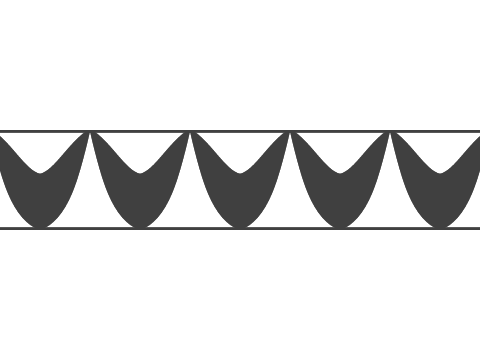
\includegraphics[width=.6\textwidth]{ansFv.png}
      \end{center}
    \end{enumerate}
  \end{freeResponse}
\end{question}
\mynewpage



\begin{question}
  Sometimes, frieze patterns with horizontal-reflections are unavoidable.
  \begin{enumerate}
  \item Can you find a frieze pattern that has symmetry through
    glide-reflections and $180^\circ$ rotations but not through
    horizontal-reflections? If YES, show me such a frieze pattern. If
    NO, explain why not.
  \item Can you find a frieze pattern that has symmetry through
    glide-reflections and horizontal-reflections but not through
    $180^\circ$ rotations? If YES, show me such a frieze pattern. If
    NO, explain why not.
  \end{enumerate}
    
  \begin{freeResponse}
    \begin{enumerate}
    \item NO, this cannot be done.
      \begin{itemize}
      \item First think about the $180^\circ$ rotation. This means
        that the lower-half and top-half of the frieze pattern look
        the same, but they may be in opposite directions/orientations.
      \item Next think about symmetry through glide-reflections. This
        means that the orientations of the top-half and lower-half
        must be the same (though possibly shifted).
      \end{itemize}
      Since the direction/orientation of both the top-half and the
      lower-half of the frieze pattern is the same, we must also have
      symmetry through horizontal-reflections.
    \item NO, this cannot be done.
      \begin{itemize}
      \item First think about the horizontal-reflection. This means
        that the frieze pattern is its own mirror image across a
        vertical line. 
      \item Next think about symmetry through glide-reflections. This
        means that the orientations of the top-half and lower-half
        must be the same (though possibly shifted).
      \end{itemize}
      Putting this together, we see that the lower-half and top-half
      of the frieze pattern look the same, and have no orientation
      other than a shift. Hence the frieze pattern must also have
      symmetry through $180^\circ$ rotations.
    \end{enumerate}
  \end{freeResponse}
\end{question}
\mynewpage


%% BAD BAD THIS IS THE SUMMARY QUESTION... JUST CONNECT TO BEGINNING
\begin{question}
  DISPLAY a SINGLE frieze pattern that has simultaneously has symmetry
  through 
  \begin{itemize}
  \item translations,
  \item glide-reflections,
  \item vertical-reflections,
  \item $180^\circ$ rotations, and
  \item horizontal-reflections.
  \end{itemize}
  \begin{freeResponse}
    Here it is:
    \begin{center}
      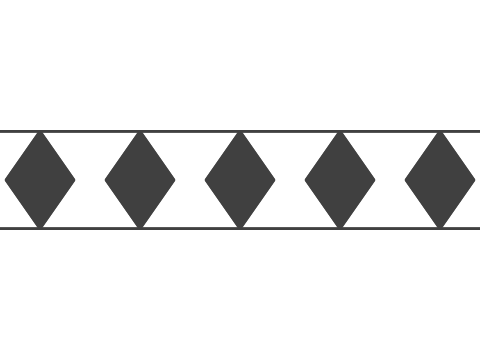
\includegraphics[width=.6\textwidth]{ansTGV8H.png}
    \end{center}
  \end{freeResponse}
\end{question}





\end{document}
